\documentclass[a4paper,oneside]{Tptesi2}

\usepackage[italian]{babel}
\usepackage{listings}
\usepackage{amsmath,amssymb}
\usepackage{verbatim}
\usepackage{indentfirst}
\usepackage[utf8]{inputenc}
\usepackage{subfigure}
\usepackage{algorithmic}
\usepackage{framed}
\usepackage{rotating}
\usepackage{cite}
\usepackage{url}
\usepackage{hyperref}

% Packages -----------------------------------------------------------------------
%\usepackage{amsthm}
%\usepackage{amsmath}          % Non necessario se usi TPTESI2 perche' gia` incluso
%\usepackage[dvips]{graphicx}  % Non necessario se usi TPTESI2 perche' gia` incluso
%\usepackage{url} %non usare se si usa hyperref


\newcommand{\mr}{\emph{motore di ricerca}}
\newcommand{\Mr}{\emph{Motore di ricerca}}
\newcommand{\ws}{Web~service }


% Use a small font for the verbatim environment
\makeatletter  % makes '@' an ordinary character
\renewcommand{\verbatim@font}{%
  \ttfamily\footnotesize\catcode`\<=\active\catcode`\>=\active%
}
\makeatother   % makes '@' a special symbol again
%
% Simboli Matematici -------------------------------------------------------------
%\newcommand{\h}{\mathcal{H}_\infty} % scorciatoia per sequenza usata spesso
% Definizioni & Teoremi ----------------------------------------------------------
\newtheorem{teorema}{Teorema}[chapter]
\newtheorem{corollario}[teorema]{Corollario}
\newtheorem{lemma}[teorema]{Lemma}
%\theoremstyle{definition}
\newtheorem{definizione}{Definizione}[chapter]
\newtheorem{proposizione}[definizione]{Proposizione}
% Formattazione Figure -----------------------------------------------------------
\setcounter{topnumber}{3}
\setcounter{totalnumber}{3}
\def\topfraction{1}
\def\textfraction{0}
% Fuzz ---------------------------------------------------------------------------
%\hfuzz10cm %Non scassare linee che escono dal bordo
% Frontespizio -------------------------------------------------------------------
       \title{Continual Learning : Visual Recognition per Problemi con Task Incrementali}
       \author{Lorenzo Gianassi}
       \titolocorso{Ingegneria Informatica}
       \chair{Andrew D. Bagdanov}
       \numberofmembers{1} %numero dei relatori
       \degreeyear{2019/2020}
       \numerocorrelatori{2} %numero dei correlatori
       \correlatori{insert correlators\ldots} % i correlatori separati da \\

%
% ---- Inclusioni (vedi piu` sotto per il comando "include" --------------
%\includeonly {introduzione,chapter1, chapter2}
%\includeonly {chapter1, chapter2, chapter3, chapter4, chapter5, chapter6}
%\includeonly{chapter6}
%
\hypersetup{%
%  pdfpagemode=FullScreen,%
  plainpages=false,%
  breaklinks,%
  pdftitle={},%
  pdfauthor={},%
  pdfsubject={},%
  pdfkeywords={},%
  colorlinks=false}

\begin{document}

\frontmatter

%\hyphenation{}
%
\pagestyle{headings} % rende attive le impostazioni sulla testata!
%
\maketitle % crea il frontespizio (ricordati di copiare "stemma.eps" nella tua directory)
%
%
%\pagenumbering{roman}
\tableofcontents % inserisce indice generale
\cleardoublepage
%\addcontentsline{toc}{chapter}{Elenco delle figure}
%\listoffigures   % inserisce indice figure
%\addcontentsline{toc}{chapter}{Elenco delle tabelle}
%\listoftables    % inserisce indice tabelle
%\addcontentsline{toc}{chapter}{Elenco degli algoritmi}
%\listofalgorithms
%
%--------------- Inizio del testo vero e proprio
%

%\cleardoublepage
%\pagenumbering{arabic}
%\input{files/ringraziamenti}
\frontmatter
\chapter{Introduzione}\label{ch:introduzione}
\section*{Motivazioni}
Gli esseri umani e gli animali hanno la capacità di acquisire, perfezionare e modificare continuamente le proprie conoscenze e abilità per tutta la durata della loro vita. Questa capacità, chiamata \textit{Continual Learning}, è composta da una ricca serie di meccanismi \textit{neurocognitivi} che insieme contribuiscono allo sviluppo e alla specializzazione delle nostre abilità sensomotorie, nonché al rafforzamento e al recupero della memoria a lungo termine. Di conseguenza, l'applicazione del \textit{Continual Learning} a  \textit{sistemi computazionali} e \textit{agenti autonomi} che interagiscono nel mondo reale ed elaborano flussi continui di informazioni può essere di  fondamentale importanza. Tuttavia, il \textit{Continual Learning} rimane una sfida di lunga data per il \textit{Machine Learning} e i modelli di \textit{Rete Neurale} poiché l'acquisizione continua di informazioni disponibili in modo incrementale da distribuzioni di dati non stabili generalmente porta ad ottenere il \textit{Catastrophic Forgetting}, concetto che andremo a definire successivamente.\newline
Questo rappresenta un grave problema per i modelli di \textit{Rete Neurale} moderni che in genere apprendono rappresentazioni da \textit{batch} stazionari di dati di \textit{Training}, quindi senza tenere conto delle situazioni in cui le informazioni diventano disponibili. Di conseguenza, la capacità  di apprendere da un flusso continuo  senza avere una perdita di memoria sui dati precedenti potrebbe avvicinare l'apprendimento delle \textit{reti neurali} a quello dell'essere umano con sviluppi interessanti per la scienza.
\section*{Presentazione del Lavoro}
In questo elaborato di tesi, partendo dal lavoro di \cite{Continual_Learning}, verrà descritto il concetto \textit{Continual Learning} mostrandone i pregi e le difficoltà(\textit{Catastrophic Forgetting}) tramite un problema di \textit{Visual Recognition}. Per fare ciò è stato implementato un \textit{framework} che fosse in grado di eseguire una \textit{Pipeline}, che avrà il compito di eseguire l'apprendimento svolto da un modello per il \textit{Continual Learning} mostrando l'occorrere del \textit{forgetting}. Prima di mostrare i risultati ottenuti verranno descritti i concetti a livello teorico e presentati gli strumenti utilizzati durante la \textit{Pipeline}.\newline
Il lavoro descritto è diviso in tre parti: la prima relativa al \textit{Joint-Train} e le ultime due alle configurazioni \textit{Task Agnostic/Task Aware}. Successivamente, sarà presentata una soluzione molto \textit{naïve} ispirata dal \textit{paper} \cite{Continual_Learning}.


\mainmatter
\chapter{Definizioni}\label{ch:chapter1}
In questo capitolo andiamo a introdurre i concetti principali su cui si basa l'elaborato, che ci serviranno successivamente per apprezzarne l'utilità. 
\section{Continual Learning}
Negli ultimi anni i modelli del \textbf{Machine Learning} sono stati addirittura in grado di sorpassare l'intelletto umano per svariati problemi, come ad esempio il \textbf{Visual Recognition}.
Sebbene questi risultati siano sorprendenti, sono stati ottenuti con modelli statici non in grado di espandere il loro comportamento o adattarlo nel tempo. Si introduce quindi il concetto del \textbf{Continual Learning} su cui si basa questo elaborato.\newline
\textit{Continual Learning} mira a creare algoritmi di\textit{Machine Learning} in grado di accumulare un insieme di conoscenze apprese sequenzialmente. L'idea generale alla base di quest'ultimo è rendere gli algoritmi in grado di apprendere da una fonte di dati reale. In un ambiente naturale le opportunità di apprendimento non sono disponibili contemporaneamente e devono essere elaborate in sequenza.\newline
Il \textbf{Continual Learning} studia il problema dell'apprendimento da uno \textit{stream} infinito di dati, con l'obbiettivo di estendere gradualmente la conoscenza e di usarla per allenamenti successivi. La dimensione dello \textit{stream} di dati ed il numero di \textit{tasks} su cui si lavora non è necessariamente noto a priori.  Il \textit{Continual Learning} può essere anche definito come \textbf{Lifelong Learning}, \textbf{Sequential Learning} o \textbf{Incremental Learning}.
Il concetto fondamentale su cui si basa  è la natura sequenziale del processo di apprendimento, in cui solo una porzione dei dati di input di uno o più \textit{tasks} è disponibile in quell'istante di tempo.
\section{Catastrophic Forgetting}
Come viene introdotto in \cite{Continual_Learning}, una rete neurale \textit{dimentica} quando le sue prestazioni su una distribuzione dati vengono ridotte dall'apprendimento su una successiva.
La sfida maggiore del \textit{Continual Learning} consiste nell'apprendere evitando il  \textbf{Catastrophic Forgetting}, cioè la performance di previsione su dati appartenenti a \textit{tasks} precedentemente visionati nel training non dovrebbe calare nel tempo in seguito all'aggiunta di nuovi \textit{tasks}.
Definiamo adesso il \textbf{Catastriphic Forgetting}, noto anche come \textbf{Catastrophic Interference}, come la tendenza di una rete neurale artificiale a dimenticare completamente e in modo improvviso le informazioni apprese in precedenza dopo aver appreso nuove informazioni (come viene definito in \cite{Continual_Learning}).
\section{Stability-Plasticity Dilemma}
Per sopperire al \textbf{Catastrophic Forgetting} i sistemi di apprendimento devono, da una parte , mostrare la capacità di acquisire nuova conoscenza e affinare quella già esistente sulla base di un input continuativo, dall'altra, impedire alla nuova informazione di interferire con la conoscenza pregressa.
Il concetto  per il quale un sistema sia in grado di essere "\textit{plastico}" per l'integrazione di nuove informazioni e "\textit{stabile}"
in modo da non interferire \textit{catastroficamente} con la conoscenza precedentemente consolidata è definito con il nome \textbf{Stability-Plasticity Dilemma}.\newline
Come viene descritto in \cite{stability/plasticity} , troppa "plasticità" farà sì che i dati precedentemente codificati siano costantemente dimenticati, mentre troppa "stabilità" impedirà la codifica efficiente di questi dati a livello delle sinapsi.
\section{Task Agnostic-Task Aware}
Un concetto importante su cui si basa l'esecuzione del mio programma che simula il \textbf{Continual Learning} è la dualità di approccio \textbf{Task-Agnostic/Task-Aware}.
Definiamo un approccio \textbf{Task-Agnostic} quando la rete non conosce bene i limiti dei \textit{tasks}, cioè non conosciamo a quale \textit{task} appartenga la \textit{label} del dato in input alla \textbf{Rete Neurale Convoluzionale}. Mentre, nell'altro caso, l'approccio  \textbf{Task-Agnostic} è contraddistinto dalla nozione del \textit{task} corrente a cui appartiene il dato in input.\newline
Questi due approcci ci consentono di ottenere risultati diversi sotto l'aspetto dell'\textit{accuracy} della rete, sia durante che al termine del ciclo previsto per vedere tutti i \textit{tasks}. In particolar modo noi possiamo avere per entrambi sia il processo di \textbf{training} che quello di \textbf{testing}, ottenendo sostanzialmente quattro combinazioni di possibili processi.\newline
Vedremo successivamente come sarà possibile simulare queste due tipologie di \textit{training/testing} tramite il metodo \textit{set\_tasks} della classe che rappresenta la 
\textbf{rete neurale convoluzionale}.

\chapter{Componenti del Progetto}\label{ch:chapter2}
In questo capitolo verranno mostrati gli strumenti utilizzati per la creazione del \textit{framework}, che riproduce l'apprendimento del \textit{Continual Learning}.
\section{PyTorch}
\textbf{PyTorch} è una libreria di \textit{Machine Learning} open source basata sulla libreria \textbf{Torch}, utilizzata per applicazioni come la visione artificiale e l'elaborazione del linguaggio naturale, sviluppata principalmente dal laboratorio di ricerca AI di Facebook. È un software gratuito e open source nato  per essere utilizzato con il linguaggio di Programmazione Python(come avviene in questo elaborato), ma presenta  anche un'interfaccia C ++.
È stata utilizzata questa libreria perchè fornisce due specifiche molto utili per lavorare con le Reti Neurali: \textit{Pytorch Tensor} e i Moduli (AutoGrad ,Optim, nn).
PyTorch definisce una classe chiamata \textit{Tensor} (torch.Tensor) per memorizzare e operare su array di numeri rettangolari multidimensionali omogenei.
\newpage
\subsection{PyTorch Tensor}
I tensori PyTorch sono simili agli array NumPy, ma possono essere utilizzati anche su una GPU Nvidia compatibile con CUDA. Per lavorare al \textbf{Visual Recognition} è molto utile l'utilizzo della GPU: i tempi e le perfomance ne risentono in positivo.
\subsection{Moduli}
PyTorch utilizza un metodo chiamato \textit{automatic differentiation} (\textbf{AutoGrad Module}). Un \textit{Recorder} registra le operazioni eseguite, quindi le riproduce all'indietro per calcolare i gradienti. Questo metodo è particolarmente potente quando si costruiscono reti neurali per risparmiare tempo in un'epoca calcolando la differenziazione dei parametri nel passo del \textit{Forward}.
\newline
Il secondo Modulo che ci interessa è \textbf{Optim Module}(\textit{torch.optim}).
È un modulo che implementa vari algoritmi di ottimizzazione utilizzati per la creazione di reti neurali. La maggior parte dei metodi più usati sono già supportati, quindi non è necessario crearli da zero. In particolare l'algoritmo di \textit{ottimizzazione} che è stato scelto in questo elaborato è \textit{optim.SGD}, il quale implementa lo \textit{stochastic gradient descent}.
Durante il \textit{training} si adotteranno i metodi della classe \textit{optim} come \textit{ .zero\_grad()} e successivamente \textit{.step()} per fare l'update dei parametri della rete.
\newline
Infine abbiamo il modulo \textbf{\textit{torch.nn}} che ci fornisce molte più classi  per implementare e addestrare la \textit{rete neurale}. In particolare ci aiuta nella definizione della \textit{rete neurale}, e in quella dei \textit{layers} che la formano.
\newpage
I \textit{Packages} utilizzati in questo elaborato sono:
\begin{itemize}
    \item \textit{torch.nn.Module}: è una classe base per tutti i moduli di \textit{Rete Neurale}
    \item \textit{torch.nn.Linear}: utilizzato per i  \textit{layer Fully Connected}
    \item \textit{torch.nn.Conv2d}: utilizzato per i \textit{Layer Convoluzionali}
    \item \textit{torch.nn.MaxPool2d}: utilizzato per applicare un max pooling 2D 
    \item \textit{torch.nn.ReLU}: funzione di attivazione dei \textit{layer}
    \item \textit{torch.nn.CrossEntropyLoss}: funzione per il calcolo della \textit{Loss} della rete
\end{itemize}
Tutte le nozioni su \textit{Pytorch} e sui suoi \textit{Module} e  sui \textit{Tensori} sono stati presi come riferimento i \textit{docs} di \textit{PyTorch} \cite{pytorch}, \cite{pytorch_datasets} e \cite{pytorch_optim}.
\section{Dataset} 
\subsection{CIFAR-10}
Il dataset utilizzato in questo elaborato è \textbf{CIFAR-10}.
Esso è costituito da 60000 immagini a colori (avranno 3 canali per ciascuna immagine per gestire l'RGB) 32x32 divise in 10 classi, con 6000 immagini per classe. Sono disponibili 50000 immagini di allenamento e 10000 immagini di prova, come viene descritto in \cite{Cifar}.\newline
Il dataset è suddiviso in cinque \textit{batches} di Training e un batch di \textit{testing}, ciascuno con 10000 immagini. Il \textit{batch} di prova contiene esattamente 1000 immagini selezionate casualmente da ciascuna classe. I \textit{batches} di \textit{training} contengono le immagini rimanenti in ordine casuale, ma alcuni di essi possono contenere più immagini di una classe rispetto a un'altra. In  particolare, i \textit{batches} di \textit{training} contengono esattamente 5000 immagini di ciascuna classe.
\newpage
In questa immagine possiamo notare le dieci \textbf{classi} di \textbf{CIFAR-10} oltre a dieci esempi presi in maniera casuale da ciascuna classe.
\begin{figure}[ht]
\centering
\caption{Classi di CIFAR-10}
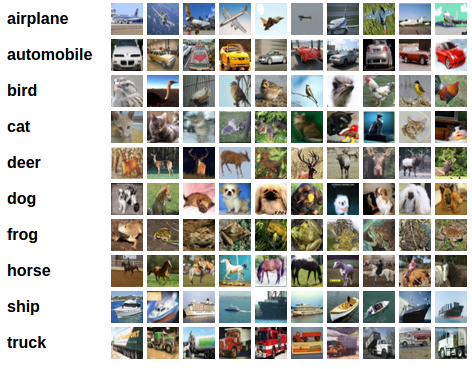
\includegraphics[width=\linewidth]{img/CIFAR.png}
\label{figure : CIFAR-10}
\end{figure}

\subsection{Gestione del Dataset}
Alla base della gestione dei \textbf{}{dataset} vi è la classe \textit{torch.utils.data.DataLoader}.
In particolare tutti  sono sottoclassi di torch.utils.data.Dataset, ovvero presentano  i metodi \textit{getitem()} e \textit{len()} implementati.
\newline
Per gestire il dataset \textbf{CIFAR-10} è stato istanziato nel progetto una classe \textit{Filtered\_dataset} che si occupasse di questa mansione.
L'obbiettivo dell'elaborato era rappresentare il problema del \textbf{Continual Learning} e per fare ciò è stato necessario dividere il dataset utilizzato in \textbf{\textit{tasks}}.
Ciò significa che a seconda del numero di \textit{tasks} che si vuole utilizzare per simulare il \textbf{Continual Learning}
sarà diviso il dataset per \textit{labels}. Ad esempio se si volesse utilizzare 5 \textit{tasks},  ognuno di essi conterrebbe 2 \textit{labels}.\newline
La classe \textit{Filtered\_dataset} si occupa di creare dei \textbf{subsets} con con il metodo della libreria di \textbf{PyTorch} \textit{torch.utils.data.Subset} che crea quest'ultimi dal dataset originario, supportato dal metodo \textit{idx\_tasks} (usato per la divisione delle \textit{Labels} nei \textit{tasks}).
Nel processo di suddivisione del dataset è stato necessario \textit{"mappare"} le \textit{labels} del dataset in modo tale da essere coerenti con l'output della rete. In particolare ciò è stato fatto tramite due attributi della classe \textit{Filtered\_dataset}:\textit{original2task} e \textit{task2original}. Questi due attributi consistono in due dizionari con chiave-valore, le \textit{labels} e la rispettiva mappatura.
Si reso inoltre possibile \textit{randomizzare} le \textit{labels} all'interno di ciascun \textit{task} per poter fare ulteriori \textit{tests} con il metodo \textit{idx\_tasks}.
\newline
\section{Rete Neurale Convoluzionale}
La \textbf{Rete Neurale Convoluzionale} (CNN o ConvNet) è una classe di \textit{reti neurali} profonde, molto spesso  applicata all'analisi ed al riconoscimento delle immagini.
La \textbf{Rete Neurale Convoluzionale} utilizzata in questo progetto è formata da sei \textit{Conv2D} layers separati da due \textit{MaxPool2D} ed infine da due \textit{Fully Connected Layer} sui cui ho applicato \textit{Dropout} per limitare l'\textit{overfitting} durante il \textit{training}. Per la scelta della conformazione della rete e per le definizioni delle tipologie dei vari \textit{layers} ho seguito il libro \cite{DeepLearningPython} e i docs di \textit{PyTorch}.
La particolarità di questa rete è che il \textit{layer} dell'output è \textbf{\textit{Dinamico}}, cioè che cambia a seconda del numero di \textit{tasks} su cui si vuole lavorare e sulla tipologia di approccio scelto tra \textit{Task-Agnostic} e \textit{Task-Aware}.
In particolare è possibile aggiungere nuovi \textit{layers} di output con il metodo\textit{add\_task} che richiama semplicemente il metodo \textit{add\_module} della classe \textit{nn.Module}.
Un altro metodo importante della \textit{rete neurale} sarà  \textit{set\_tasks} che  permette di settare il numero di \textit{tasks} voluti come output. I due attributi fondamentali della classe \textit{net} sono \textit{task\_fcs} e \textit{current\_tasks}, che sono sostanzialmente due \textit{array} contenenti gli indici dei \textit{tasks}. Il primo conterrà tutti i \textit{layers} lineari per le varie  \textit{Classification Head}, mentre il secondo, seleziona quale(i) task(s) sono correntemente attivi.
Qui di seguito si illustra la \textit{rete neurale} per un singolo \textit{task} con tutte le classi corrispondenti al \textit{Joint Training}:
Net(\\
  (conv1): Conv2d(3, 32, kernel_size=(3, 3), stride=(1, 1), padding=(1, 1))\\
  (conv2): Conv2d(32, 64, kernel_size=(3, 3), stride=(1, 1), padding=(1, 1))\\
  (conv3): Conv2d(64, 64, kernel_size=(3, 3), stride=(1, 1), padding=(1, 1))\\
  (pool): MaxPool2d(kernel_size=2, stride=2, padding=0, dilation=1, ceil_mode=False)\\
  (conv4): Conv2d(64, 128, kernel_size=(3, 3), stride=(1, 1), padding=(1, 1))\\
  (conv5): Conv2d(128, 128, kernel_size=(3, 3), stride=(1, 1), padding=(1, 1))\\
  (conv6): Conv2d(128, 256, kernel_size=(3, 3), stride=(1, 1), padding=(1, 1))\\
  (fc1): Linear(in_features=16384, out_features=120, bias=True)\\
  (fc2): Linear(in_features=120, out_features=84, bias=True)\\
  (dropout): Dropout(p=0.5, inplace=False)\\
  (task0\_fc): Linear(in_features=84, out_features=10, bias=True) )

\newpage
Il \textit{layer} \textit{Task0\_fc} è l'ultimo che è stato aggiunto con \textit{add\_task} e \textit{settato} con \textit{set\_task}.
Se l'esperimento fosse stato condotto su più \textit{tasks} ci sarebbero stati altri \textit{layers} oltre a \textit{Task0\_fc}. Nel caso in cui l'output voluto fosse stato su più tasks, nel metodo \textit{Forward} della rete tramite \textit{torch.cat}, sarebbero stati concatenati tra di loro i parametri corrispondenti selezionati da \textit{current\_tasks}.
\newline
La \textit{Funzione di Attivazione} utilizzata nei  \textit{layers convoluzionali} è \textbf{ReLu}, come anticipato precedentemente.
La \textbf{rectified linear activation function} o \textbf{ReLU} in breve è una funzione lineare a tratti che darà  come output direttamente l'input se è positivo, altrimenti produrrà zero. L'utilizzo della \textbf{ReLu} consente di ottenere un \textit{training} e una performance migliori.
\newline
Per quanto riguarda la funzione che si occupa del calcolo della \textit{Loss} è stata selezionata la \textbf{CrossEntropyLoss}. Questa funzione combina in una unica classe \textit{nn.LogSoftmax()} e \textit{ nn.NLLLoss()}.
Come anticipato nel paragrafo relativo a \textbf{PyTorch} è stato utilizzato come \textit{optimizer} \textbf{SGD} con \textit{Learning Rate} pari a  \mathbf{0.001}.\newline
Infine, è stato reputato necessario applicare \textbf{Dropout} ai due \textit{Fully Connected Layer} che precedono il \textit{layer} di output dinamico. Durante il \textit{training} azzera in modo casuale alcuni degli elementi del tensore di input con probabilità \textit{p} utilizzando campioni da una distribuzione di Bernoulli. In questo modo è stata ottenuta una diminuzione dell'\textit{overfitting}  riscontrato nella \textit{rete}.
\chapter{Esperimenti}\label{ch:chapter3}
\section{Introduzione al Progetto}
Prima di poter iniziare a mostrare il progetto è necessario porre delle basi e limiti per quest'ultimo.
Per analizzare il concetto del \textbf{Continual Learning} ci concentreremo sul problema di \textit{classificazione}, tipico del \textit{Deep Learning}. La classificazione implica la previsione a quale classe appartenga un elemento. Alcuni classificatori sono binari, altri sono multi-classe, in grado di discernere un esempio in una delle diverse classi. Noi, quindi, ci andremo a concentrare sull'utilizzo di un classificatore \textit{multi-classe}.
\newline
La seconda limitazione riguarda l'approccio \textbf{\textit{Task Incremental}}.
\newline Il \textbf{\textit{Task Incremental}} corrisponde ad un approccio in cui i dati arrivano in sequenza di \textit{batches} e ognuno dei quali corrisponde ad un \textit{task}. Ad ogni \textit{task} corrisponderà un nuovo insieme di \textit{labels} il cui numero dipenderà dalla quantità di quest'ultime nel \textit{dataset} e dalla loro divisione scelta. In altre parole, assumiamo  che per un dato \textit{task}, tutti i dati diventino disponibili simultaneamente seguendo il concetto di \textit{Training Offline}. Ciò consente un \textit{training} per più epoche su tutti i suoi dati di addestramento, mescolati ripetutamente per garantire delle condizioni di 
\textit{i.i.d.}. È importante sottolineare che i dati appartenenti al  precedente o al futuro \textit{task}
non saranno utilizzabili. Ottimizzare/Allenare per un nuovo \textit{task} in questa configurazione si tradurrà nel \textit{\textbf{Catastrophic Forgetting}}, con significativi
cali sulle prestazioni relative ai vecchi \textit{tasks}, salvo siano adottate strategie specifiche.
\newline 
A differenza della limitazione alla configurazione \textit{Multi-Head} utilizzata nel paper\cite{Continual_Learning},
in questo elaborato proveremo ad analizzare entrambe le configurazioni \textit{Multi-Head/Single-Head}. Ciò corrisponde ai due approcci che abbiamo già introdotto nel primo capitolo: \textbf{Task-Agnostic/Task-Aware}. Nel caso di \textbf{Task-Agnostic} avremo una  \textit{Single-Head} per tutti i \textit{tasks} perchè non è noto su quale stiamo facendo \textit{training/testing}, mentre per \textbf{Task-Aware} avremo una \textit{Multi-Head} e selezioneremo l'\textit{Output} corrispondente a quello corrente.
\section{Pipeline}
Per simulare il processo di \textbf{Continual Learning} è stato necessario stabilire una \textit{Pipeline} che avrebbe dovuto seguire l'algoritmo. A seconda delle tipologie di approccio 
\textbf{Task-Agnostic/Task-Aware} avremo delle differenze all'interno della \textit{Pipeline} che verranno analizzate successivamente.
\newline
Per descrivere al meglio il problema del \textit{Catastrophic Forgetting} è stato valutato di dividere il dataset in 5 \textit{tasks} ciascuno con i dati relativi  a due \textit{labels}, visto che \textit{CIFAR-10} ha 10 classi. Se fossero stati utilizzati solamente due \textit{tasks} si sarebbero potuti ottenere dei risultati poco significativi per il progetto.
\newpage
La \textbf{\textit{Pipeline}} del processo è la seguente:
\begin{enumerate}
    \item Creare \textbf{\textit{Rete Neurale Convoluzionale}}  che farà da \textit{Backbone};
    \item Per ogni t in \textit{Tasks}:
    \begin{enumerate}
        \item Aggiungere un nuovo \textit{Classification Module} per il \textit{task} corrente;
        \item \textit{SetTask} per selezionare l'\textit{output} corretto della rete a seconda di  \textit{Aware/Agnostic Training}; 
        \item Fare il \textit{Training} per il \textit{Task} t;
        \item \textit{SetTask} per selezionare l'\textit{output} corretto della rete a seconda di  \textit{Aware/Agnostic Testing};
        \item Fare \textit{Test}  per il \textit{Task} t;
     \end{enumerate}
    \item Fare \textit{Test}  per ogni \textit{task} dopo l'ultimo \textit{Training}, selezionando \textit{output} giusto per la tipologia di \textit{testing}.
\end{enumerate}
2.b/2.d/3 sono le fasi che vengono influenzate dalla scelta della tipologia di \textit{Agnostic/Aware}. Ciò consiste nel fatto che l'\textbf{output} della rete verrà modificato seguendo il paradigma \textit{Task-Aware/Task-Agnostic}, diventando unico per più \textit{tasks} nel caso \textit{Agnostic} e singolo per il \textit{task} specifico per \textit{Aware}.\newline
Inoltre, il processo della \textbf{\textit{pipeline}} sarà il medesimo sia al variare del numero di \textit{tasks} che della formazione di quest'ultimi(caso di \textit{labels randomiche}).\newline
Avremo, quindi, 5 configurazioni diverse di Processi di cui 4 andranno a combinare \textit{Aware/Agnostic outputs} e una sarà relativa al \textit{Joint-Train}.\newline
Verranno mostrati i risultati ottenuti nelle quattro configurazioni tenendo presente come \textbf{\textit{upperbound}} il valore della \textbf{\textit{accuracy}} ottenuta dal \textbf{\textit{Joint-Train}}.
\newpage
\section{Esperimenti}
Quindi le configuazioni di nostro interesse saranno:
\begin{enumerate}
     \item \textbf{\textit{Joint-Training/Testing}}: Corrisponde sostanzialmente ad allenare e testare la rete su tutte le \textit{labels} contemporaneamente. Sarà equivalente ad un unico \textit{Task} con tutti gli \textit{examples} del dataset.
    
    \item \textbf{\textit{Task-Agnostic Training}/\textit{Task-Agnostic Testing}}: \textit{training} con \textit{output} per ogni \textit{task}, \textit{testing} con \textit{output} per ogni \textit{task}.  
    
    \item \textbf{ \textit{Task-Agnostic Training}/\textit{Task-Aware Testing}} : \textit{training} con \textit{output} per ogni \textit{task}, \textit{testing} con \textit{output} per \textit{task} specifico.
    
    \item \textbf{\textit{Task-Aware Training}/\textit{Task-Aware Testing}} : \textit{training} con \textit{output} per \textit{task} specifico, \textit{testing} con \textit{output} per \textit{task} specifico. 
    
    \item \textbf{\textit{Task-Aware Training}/\textit{Task-Agnostic Testing}}: \textit{training} con \textit{output} per \textit{task} specifico, \textit{testing} con \textit{output} per ogni \textit{task}  
\end{enumerate}
Per comprendere nel miglior modo i risultati saranno  rappresentate le \textit{accuracies} delle configurazioni in due grafici. Il primo sarà relativo al \textbf{\textit{Task-Agnostic Training}} riportando le \textit{accuracies} relative ai casi \textit{Aware/Agnostic} così da visualizzare le differenze, mentre il secondo avrà \textit{Task-Aware Training}. Entrambi i grafici saranno confrontati al valore \textit{Joint-Train} che rappresenterà l'\textit{upperbound} per qualsiasi configurazione. \newline
Un altro valore importante da analizzare per comprendere al massimo il valore del \textit{Catastrophic Forgetting} è la differenza tra la media delle \textit{accuracies} dopo l'allenamento relativo a ciascun \textit{task} e quella dopo l'ultimo \textit{task}. Questo valore ci fornisce il \textbf{\textit{Catastrophic Forgetting}} a cui siamo andati incontro grazie al \textit{Continual Learning}.
\newpage
\subsection{Joint-Training}
Prima di andare ad analizzare le varie configurazioni è necessario concentrarci sul \textbf{\textit{Joint-Training}}.
Il \textbf{\textit{Joint-Training}} corrisponde al generico procedimento di \textit{Training/Testing} che viene eseguito nel \textit{Visual Recognition}. Ciò consiste in un addestramento e \textit{testing} fatto sulla totalità degli esempi appartenenti ai \textit{batches} che compongono il dataset senza considerare la divisione in \textit{Tasks} ignorando, quindi, il paradigma del \textit{Continual Learning}. Questa \textit{baseline} ci fornisce un \textit{upperBound} per le \textit{accuracies} rilevate.
Il valore di \textit{accuracy} che abbiamo ottenuto dal nostro \textit{Joint-Training} è di \textit{\textbf{77.6}} e lo utilizzeremo come riferimento nei nostri grafici. 
\subsection{Agnostic-Training}
Qui di seguito  viene riportato il grafico con i risultati ottenuti sia per \textit{Agnostic} che \textit{Aware Testing}: 
\begin{figure}[ht]
\centering
\caption{Agnostic Training}
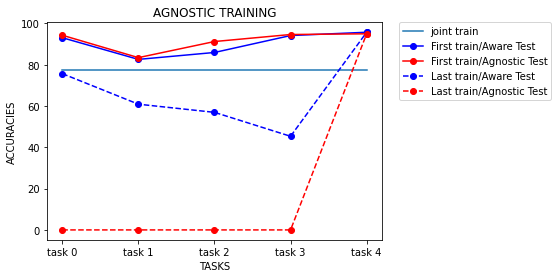
\includegraphics[width=\linewidth]{img/Agnostic_Agnostic-Aware.png}
\label{figure : Angostic_training}
\end{figure}
\newpage
Prima di analizzare il grafico  andiamo a considerare il paradigma l'\textit{Agnostic-Training} che consiste nel \textit{training}
senza sapere di quale \textit{task} ci stiamo occupando.
Ciò comporta che ad ogni \textit{task} l'\textit{output} della rete consisterà in tutti i moduli dei \textit{tasks} fino a quello corrente concatenati nel metodo \textit{Forward}, questo perchè non possiamo selezionare l'\textit{output} relativo al \textit{Task} in esecuzione.
\newline
Dal grafico ~\ref{figure : Angostic_training}, che si trova a pagina precendete, possiamo notare vari aspetti interessanti sui risultati ottenuti. Prima di tutto, notiamo che i valori delle \textit{accuarcies} sui vari \textit{tasks}, calcolate dopo i rispettivi \textit{Training}, ottengono valori molto elevati che superano persino il valore del \textit{Joint-Training}. Questo è dovuto al numero minore di dati utilizzati rispetto al dataset completo e dal fatto che il \textit{test} è effetuato subito  dopo il \textit{training} del relativo \textit{task}. Inoltre, da notare come i due approcci di \textit{testing} ottengano \textit{accuracies} quasi identiche: la rete viene \textit{testata} subito dopo il \textit{train} relativo di conseguenza i pesi associati alla clasificazione sono molto precisi per entrambe le configurazioni, ottenendo risultati per ciascun \textit{task} migliori anche del \textit{Joint-Training} .
L'\textit{accuracy} calcolata sull'ultimo \textit{task}, naturalmente, avrà valore uguale per tutte e quattro le configurazioni, come si può notare nel grafico ~\ref{figure : Angostic_training} nel punto relativo a quest'ultimo.
\newline
Per quanto riguarda le \textit{accuracies} calcolate successivamente all'ultimo \textit{training}, vediamo che si ottiene un calo drastico di precisione su ciascun \textit{Task} escluso l'ultimo come abbiamo precedentemente affermato. Questo è il fenomeno del \textbf{Catastrophic Forgetting}, introdotto nel \autoref{ch:chapter1}, che porta il \textit{modello} a dimenticare tutti i \textit{weight} relativi ai \textit{tasks} precedenti.
In particolare nella configurazione \textit{Aware} si ottengono dei valori migliori dati dall'output più preciso e specifico per il relativo \textit{task}, dati dalla selezione della \textit{Classification Head} relativa a quest'ultimo. Per quanto riguarda la configurazione di \textit{Agnostic Testing}, otteniamo un valore molto alto per l'ultimo \textit{Task} mentre per i 4 precedenti l'\textit{accuracy} cala a 0. Questo fenomeno prende il nome di 
\textit{\textbf{Task Recency Bias}}. Si tratta di un fenomeno che consiste nel fatto che la \textit{rete} abbia la tendenza a ricordare e a prevedere meglio dati su cui è stato fatto per ultimo il \textit{training} portando a dimenticare totalmente i \textbf{parametri} appartenenti ai \textit{tasks} precedenti, come viene descritto in \cite{Task_Recency_Bias}. Questo risultato è ricondotto all'utilizzo di \textit{CrossEntropyLoss}  che aumenta il valore della probabilità relativa alla classe corretta e diminuisce quella relativa alla classe non corretta all'interno della distribuzione di probabilità, dato che grazie al \textit{SoftMax} la somma dei valori deve essere uguale a uno. Ad ogni esempio del \textit{batch} del \textit{task} corrente riduce la probabilità delle classi appartenenti a quelli precedenti, andando incontro al \textbf{Catastrophic Forgetting}.
\newline
Per questo motivo è interessante valutare le medie delle \textit{accuracies} per analizzare l'occorrere del \textbf{Catastrophic Forgetting} nelle varie configurazioni.
Qui di seguito i valori delle \textit{accuracies} sono  riportate in due tabelle, una per tipologia di \textit{testing}.
\begin{table}[!htb]
\begin{minipage}{.5\linewidth}
    \centering

    \label{tab:Agnostic-Agnostic }

    \medskip

\begin{tabular}{l*{6}{c}r}
Tasks   & First Train & Last Train\\
\hline
   Task 0      &     94.30      &      0.0\\
   Task 1      &     83.45      &      0.0\\
   Task 2      &     91.25      &      0.0\\
   Task 3      &     94.65      &      0.0\\
   Task 4      &     95.00      &      95.00\\
\end{tabular}
\caption{Agnostic-Agnostic}
\label{tab:Agnostic-Agnostic}
\end{minipage}\hfill
\begin{minipage}{.5\linewidth}
    \centering

    \label{tab:Agnostic-Aware}

    \medskip

\begin{tabular}{l*{6}{c}r}
Tasks   & First Train  & Last Train\\
\hline
   Task 0      &     93.10      &      75.70\\
   Task 1      &     82.60      &      60.90\\
   Task 2      &     85.95      &      56.95\\
   Task 3      &     94.15      &      45.35\\
   Task 4      &     95.75      &      95.75\\
\end{tabular}
\caption{Agnostic-Aware}
\label{tab:Agnostic-Aware}
\end{minipage}
\end{table}
\newline
Nelle tabelle~\ref{tab:Agnostic-Agnostic} e~\ref{tab:Agnostic-Aware} notiamo, come avevamo già fatto nel grafico in figura ~\ref{figure : Angostic_training} a pagina ~\pageref{figure : Angostic_training}, che l'\textit{accuracy} della configurazione \textit{Agnostic-Agnostic} è peggiore rispetto a quella di \textit{Agnostic-Aware}, ma per valutare la differenza di valori, ma soprattutto il \textit{forgetting}, calcoliamo la media di quest'ultimi.
\newline
Facendo le medie otteniamo i seguenti valori:
\begin{itemize}
    \item Tabella~\ref{tab:Agnostic-Agnostic}: Abbiamo una \textit{accuracy} iniziale di 91.73\% e finale di 19.0\%, quindi otteniamo un decremento del 72.71\%.
    \item Tabella~\ref{tab:Agnostic-Aware}: Abbiamo una \textit{accuracy} iniziale di 90.30\% e finale di 66.92\%, quindi otteniamo un decremento del 23.38\%.
\end{itemize}
Notiamo che la media dell'\textit{accuracies} del \textit{Task Agnostic} e \textit{Task Aware Testing} sono entrambe inferiori dell'\textit{upperbound} rappresentato dal \textit{Joint-Train}, confermando ciò che si poteva notare già a livello grafico nell'immagine~\ref{figure : Angostic_training}.
Il decremento della \textit{accuracy} ci serve a valutare l'entità del \textit{Catastrophic Forgetting} a cui siamo andati incontro.
\newline
Questo valore inoltre ci conferma il \textit{forgetting} molto elevato che abbiamo ottenuto sui \textit{tasks} precedenti all'ultimo  utilizzando la configurazione \textit{Agnostic-Agnostic}. Vedremo successivamente una soluzione \textit{naïve} al problema del \textit{Task Recency Bias}, basato sull'approccio \textit{Replay Based Methods}.
\newline
In generale, il decremento di \textit{accuracy} per entrambe le configurazioni utilizzate in questo paragrafo è elevato, anche se con entità diverse. Inoltre la distanza di \textit{accuracy} in media dal valore ottenuto con il \textit{Joint-Train} assume un valore del 10,68\%, per la configurazione \textit{Agnostic-Aware}, 58,60\% per \textit{Agnostic-Agnostic}. Questo ci fa comprendere l'entità del \textit{drop} di \textit{accuracy} a cui si può andare incontro adottando una divisione in \textit{tasks} dovuto al \textit{Catastrophic Forgetting}.
\subsection{Aware-Training}
In questa sezione ci concentriamo su altre due configurazioni\textit{Task-Aware} per il \textit{training} introdotte già a \textit{pag.}14.
A differenza della configurazione \textit{Task-Agnostic} possiamo selezionare la \textit{Classification-Head} relativa al \textit{Task} corrente: di conseguenza il \textit{Training} per ognuno di essi sarà eseguito con un \textit{output} di soli due valori modificando, quindi, l'aggiornamento dei parametri della \textit{Rete}.\newline
Riportiamo qui di seguito il grafico che rappresenta le \textit{accuracies}:
\begin{figure}[ht]
\centering
\caption{Agnostic Training}
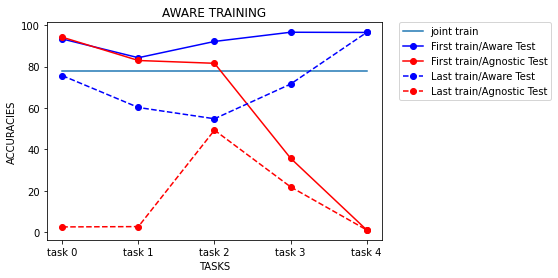
\includegraphics[width=\linewidth]{img/Aware_Agnostic-Aware.png}
\label{figure : Aware_Training}
\end{figure}
\newline
Dalla figura ~\ref{figure : Aware_Training} possiamo notare che l'andamento generale delle \textit{accuracies} segue, in linea generale, quello della figura ~\ref{figure : Angostic_training} a pagina 15.
Di conseguenza rileviamo che l'\textit{accuracy} su un \textit{task} calcolata subito dopo il corrispondente addestramento ha un valore molto buono, che in media è addirittura superiore al \textit{Joint-Train}  per \textit{Aware-Test}. Per \textit{Agnostic-Test}, invece, tende a calare all'aumentare del \textit{task}. Inoltre abbiamo che l'\textit{accuracy} sull'ultimo \textit{task} ha lo stesso valore per tutti i casi riportati, tranne uno: \textit{Aware-Agnostic}. Si può notare che l'\textit{accuracy} calcolata sull'ultimo \textit{task} a seconda della tipologia assume dei valori diversi.
In particolare per la configurazione \textit{Agnostic Test} notiamo che l'\textit{accuracy} subito dopo il \textit{Training} assume un valore sempre minore fino all'ultimo \textit{task} in cui è quasi nulla. Questo risultato è ottenuto perchè durante la fase \textit{train} utilizziamo la \textit{Classification-head} specifica del \textit{task} mentre nella fase di \textit{Testing} utilizziamo un \textit{output} unico per tutti \textit{tasks} fino a quello corrente.
Adesso mostriamo di seguito le tabelle con le \textit{accuracies} ottenute per poter capire il \textit{forgetting} ottenuto e comparare i risultati con l' \textit{Agnostic-Train}:
\begin{table}[!htb]
\begin{minipage}{.5\linewidth}
    \centering

    \label{tab:Aware-Agnostic }

    \medskip

\begin{tabular}{l*{6}{c}r}
Tasks   & First Train & Last Train\\
\hline
   Task 0      &     94.15      &       2.50\\
   Task 1      &     82.90      &       2.65\\
   Task 2      &     81.55      &      49.25\\
   Task 3      &     35.70      &      21.85\\
   Task 4      &      1.05      &       1.05\\
\end{tabular}
\caption{Aware-Agnostic}
\label{tab:Aware-Agnostic}
\end{minipage}\hfill
\begin{minipage}{.5\linewidth}
    \centering

    \label{tab:Aware-Aware}

    \medskip

\begin{tabular}{l*{6}{c}r}
Tasks   & First Train  & Last Train\\
\hline
   Task 0      &     93.30      &      75.60\\
   Task 1      &     84.25      &      60.20\\
   Task 2      &     92.10      &      54.75\\
   Task 3      &     96.55      &      71.50\\
   Task 4      &     96.45      &      96.45\\
\end{tabular}
\caption{Aware-Aware}
\label{tab:Aware-Aware}
\end{minipage}
\end{table}
\newline
Nelle tabelle ~\ref{tab:Aware-Agnostic} e ~\ref{tab:Aware-Aware} notiamo subito che la \textit{accuracy} rilevata nel caso di \textit{Aware-Testing} è migliore, ma consideriamo adesso le medie delle \textit{accuracies} e il \textit{forgetting} ottenuto.
\begin{itemize}
    \item Tabella~\ref{tab:Aware-Agnostic}: Abbiamo una \textit{accuracy} iniziale di 59.07\% e finale di 15.45\%, quindi otteniamo un decremento del 43.61\%.
    \item Tabella~\ref{tab:Aware-Aware}: Abbiamo una \textit{accuracy} iniziale di 92.53\% e finale di 71.7\%, quindi otteniamo un decremento del 20.83\%.
\end{itemize}
La prima cosa che rileviamo è che l'\textit{accuracy} iniziale della configurazione \textit{Agnostic-Agnostic} ha ottenuto un valore in media molto minore rispetto alle altre, dovuto all'\textit{Agnostic-Testing}.
L'\textit{accuracy} ottenuta nel caso \textit{Aware-Aware} è il miglior risultato e si avvicina a quella del \textit{Joint-Train} con uno scarto del 5,9\%. Mentre nel caso della Tabella ~\ref{tab:Aware-Agnostic} l'\textit{Accuracy} ottenuta rappresenta il "\textit{Lower-Bound}" dei risultati con uno scarto dal \textit{Joint-Train} del 62,15\%. 
\section{Soluzione Naïve}
In questa sezione andiamo ad proporre una soluzione con un \textit{naïve} al problema del \textit{Catastrophic Forgetting}. Esistono tre famiglie di soluzioni al problema del \textit{Continual Learning}, che vengono descritte in \cite{Continual_Learning}:
\begin{itemize}
    \item \textit{Replay-based methods}
    \item \textit{Regularization-based methods}
    \item\textit{Parameter isolation methods}
\end{itemize}
In questa sezione ci soffermeremo su una soluzione \textit{Naïve} della famiglia dei \textit{\textbf{replay-based methods}}. Questo approccio consiste nel memorizzare i campioni o generare \textit{pseudo-campioni}, con un modello generativo, appartenenti ai \textit{tasks} precedenti. Questi esempi  vengono riutilizzati durante l'apprendimento di un nuovo \textit{task} per alleviare il \textit{forgetting}.\newline
Il problema principale dei \textit{replay-based methods} risiede nella memoria: salvando esempi dai \textit{tasks} precedenti la memoria necessaria a ciascuna fase di \textit{training} sarà sempre maggiore. Ciò può esser ovviato utilizzando un limite di esempi possibili dai precedenti \textit{tasks}, ottenendo però una perdita di generalizzazione del rispettivo \textit{task}.
In particolare questi due metodi utilizzano una specifica tecnica di scelta degli esempi da ciascun insieme di esempi appartenenti ai \textit{tasks} precedenti.\newline
In questo elaborato, però, adotteremo una soluzione \textit{naïve} e semplificata, scegliendo gli esempi in modo \textit{randomico} senza basarci su nessuna metrica o \textit{bias}.
In particolare ci soffermeremo sul caso \textit{Agnostic-Training/Agnostic-Test} in modo tale da poter apprezzare l'aumento di \textit{accuracies} media e confrontarlo con il \textit{Joint-Train} (essendo stanzialmente della stessa tipologia di configurazione). Mostriamo, infatti, come cambia il valore delle \textit{accuracies} al variare del numero di esempi utilizzati appartenenti ai \textit{tasks} precedenti per ogni processo di \textit{training}. Partiamo dall'utilizzo dello 0.1\% degli esempi precedenti, fino ad arrivare all'1\%, andando a confrontare con il valore dei \textit{Joint-Train} che rappresenta l'\textit{UpperBound}.
Come in precedenza, andiamo a riportare di seguito il grafico:
\begin{figure}[ht]
\centering
\caption{Agnostic Replay Training}
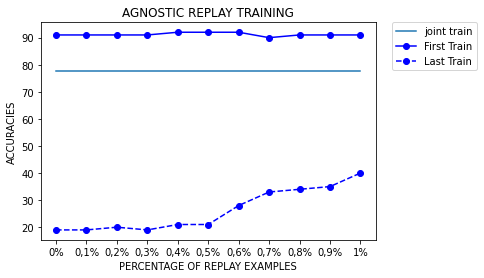
\includegraphics[width=\linewidth]{img/Agnostic_Replay.png}
\label{figure : Angostic_replay}
\end{figure}
\newline
Come si può notare dal grafico \ref{figure : Angostic_replay} all'aumentare della percentuale del numero di esempi di \textit{replay} migliora l'\textit{accuracy} in media, diminuendo il \textit{forgetting}. Tutto ciò è stato ottenuto senza l'utilizzo di nessuna strategia specifica per selezionare gli esempi ad ogni iterazione del \textit{training}. Avremmo potuto, quindi, ottenere risultati ancora migliori rispetto a quelli presentati in \ref{figure : Angostic_replay}. \newline
Inoltre aumentando il numero degli esempi utilizzati nel \textit{replay-training} dei \textit{tasks} precedenti  sarebbero stati ottenuti risultati migliori.
\newline
La scelta di questa percentuale è, però, in parte vincolata. Sarebbe stato poco rappresentativo utilizzare un numero elevato e poco intelligente da un punto di vista delle risorse di memorizzazione. Nel caso di \textit{CIFAR-10} il problema della memoria utilizzata non sussiste, ma se avessimo utilizzato un dataset dal numero di esempi  maggiore lo spazio di archiviazione assegnato agli esempi dei \textit{tasks} precedenti sarebbe stato un punto focale, essendo un punto debole dei \textit{replay-based methods}.
Ciò che si nota dal grafico \ref{figure : Angostic_replay} è che l'\textit{accuracy} ottenuta dal valore 50 dell' ascisse in poi tende a salire, mentre il valore rimane stabile intorno al 20\% nei valori delle ascisse precedenti. Possiamo, quindi,
affermare che utilizzando un numero superiore a 50 esempi per applicare il \textit{Replay Training} otterremo un miglioramento di prestazioni crescente all'aumentare di tale valore.
\newline
 La crescita comunque non è elevata e rimane  un grosso divario tra i risultati ottenuti e il valore del \textit{Joint-Train}, rimarcando nuovamente il problema del \textbf{\textit{Catastrophic Forgetting}} che affligge le rappresentazioni pratiche del \textit{Continual Learning}.


\chapter{Conclusioni}\label{ch:conclusioni}
\section{Risultati}
Il lavoro che è stato descritto in questo elaborato di tesi può essere ritenuto soddisfacente. Il nostro intento era quello di rappresentare al meglio il \textbf{Continual Learning} e il suo problema del \textbf{Catastrophic Forgetting}, perciò nella nostra \textit{pipeline} non è stato inserito nessun metodo che potesse alleviare o bloccare tale problema. Abbiamo potuto osservare come il \textit{training} effettuato in fasi diverse per ciascun \textit{task} abbia portato al \textit{forgetting}, valutandolo sia nel caso \textit{Task-Aware} che \textit{Task-Agnostic}.\newline
È stato riscontrato un \textit{forgetting} minore nelle configurazioni in cui è stato applicato il \textit{Task-Aware Test}, peggiore con \textit{Task-Agnostic Test}. Per questo motivo è stato scelto come caso interessante, su cui applicare una soluzione basata \textit{Replay-Based Methods}, \textit{Task-Agnostic Training/Task-Agnostic Test}.
Con tale soluzione è stato possibile ottenere dei risultati migliori rispetto ai precedenti. Infatti, questa configurazione soffriva del \textit{Task Rececncy Bias} che portava a dimenticare completamente i parametri dei \textit{tasks} precedenti all'ultimo visionato. Usando un numero di esempi limitato per fare il \textit{replay} siamo riusciti ad avvicinarci al \textit{Joint-Train}, mantenendo comunque un \textit{forgetting} elevato.
La rete neurale sviluppata non è ovviamente \textbf{immune} da \textbf{errori}, potrebbero essere apportate delle migliorie in modo tale da adattarsi meglio al problema in esame, ottenendo  risultati migliori.
\section{Sviluppi Futuri}
Negli esperimenti eseguiti in questo elaborato, abbiamo considerato un ambiente di apprendimento basato sul concetto \textit{Task Incremental}. In questo \textit{setting} i \textit{tasks} vengono ricevuti sequenzialmente e il \textit{Training}  viene eseguito sui dati di addestramento associati. È, quindi, richiesta la conoscenza dei limiti dei \textit{tasks} (ovvero quando i \textit{tasks} cambiano), consentendo più passaggi su grandi \textit{batch} di dati di \textit{training}. Può essere, quindi, un rilassamento del sistema di \textit{Continual Learning} desiderato che è più probabile incontrare nella pratica. Una evoluzione potrebbe essere quella di rendere il modello capace di processare dati di \textit{tasks} diversi senza considerarne i limiti, al fine di riconoscere se l'\textit{input} appartiene a un \textit{task} già osservato. Questa modifica potrebbe conferire grande flessibilità al metodo del \textit{Continual Learning} rendendolo applicabile a qualsiasi scenario in cui i dati arrivano con uno \textit{stream} infinito.
\newline
Un altro sviluppo possibile, potrebbe essere quello di utilizzare un dataset diverso. Sarebbe appunto interessante osservare i risultati all'aumentare del numero di classi presenti nel dataset, o altrimenti, all'aumentare del numero di esempi presenti nel \textit{trainset} e \textit{testset}. Un dataset che viene spontaneamente in mente dopo la lettura di questo elaborato è \textit{CIFAR-100}. Quest'ultimo non è altro che una estensione di \textit{CIFAR-10}(utilizzato in questo elaborato), composto da 100 \textit{classi} differenti. Tale modifica ci consentirebbe di visualizzare più \textit{tasks} e con un numero di classi associato maggiore.\newline
Infine, nella soluzione che abbiamo esposto per alleviare il \textit{forgetting} non è stata attuata nessuna tecnica per sceglie gli esempi su cui fare il \textit{replay}, quindi una direzione di sviluppo potrebbe essere questa. Come viene descritto in \cite{Continual_Learning}, esistono dei metodi specifici del \textbf{Reaplay Based Methods}:
\textit{iCaRL} e \textit{GEM}. In particolare, questi due metodi attuano delle politiche per la scelta degli esempi utilizzati nel \textit{replay}.
\textit{iCaRL} si basa sulla stima della \textit{Loss}, mentre \textit{GEM} si concentra sul \textit{gradiente}.

\addcontentsline{toc}{chapter}{Bibliografia}
\bibliographystyle{unsrt}
\bibliography{files/biblio}
%\bibliography{sp,xml}
%\bibliographystyle{ieeetr}
%\bibliography{sp,xml}

\end{document} 

